\section{Changes from version 1}
\label{app:changes}

Table~\ref{tab:changes} lists every claim in version 1 that this version withdraws or materially changes. Version 1 remains available on arXiv for the record.

\begin{table}[!htbp]
\centering
\caption{Claims changed between version 1 and version 2.}
\label{tab:changes}
\small
\begin{tabular}{p{0.44\textwidth}p{0.50\textwidth}}
\toprule
\textbf{Version 1} & \textbf{Version 2} \\
\midrule
GPT-oss-120B shows the highest confidence variability (SD 21.3) with near-chance discrimination (AUROC .530) and below-chance Science monitoring, a distinct failure mode. & Withdrawn. 980 of its 1{,}500 confidence values were the parser default of 50. On its 518 genuine responses AUROC is .800. The retained items are a non-random subset, and the domain profile is not interpreted (\S\ref{sec:anomalous}, Appendix~\ref{app:gptoss}). \\
\addlinespace
Within OpenAI, GPT-oss-20B outperforms the six-times-larger GPT-oss-120B, so training recipe dominates scale. & Withdrawn; it rested on the imputed values. \\
\addlinespace
DeepSeek-R1, Gemini 3.1 Pro and Qwen Think are battery-Invalid; R1 shows catastrophic inversion on the binary probe. & Corrected from arXiv:2604.17714v2. R1 is Invalid because it withdraws 95\% of its correct answers; it is not inverted. Gemini 3.1 Pro and Qwen Think are Indeterminate (blanket confidence suspected but not certifiable on 24 and 27 errors). \\
\addlinespace
Tier-level assignments are preserved across probe formats in every battery-Valid case. & Withdrawn. Battery AUROC does not predict atlas AUROC ($\rho = .00$), and three battery-Valid Gemma 3 models barely discriminate on MMLU (\S\ref{sec:probe}). \\
\addlinespace
Introduction: every Valid model in a 20-model battery sample had a domain AUROC below .55 \citep{cacioli2026c}. & Removed; it relied on the battery scoring corrected in arXiv:2604.17714v2. \\
\addlinespace
The Gemma 3 $\to$ Gemma 4 step shows that a single generational step can recover an entire class of failure modes. & Reframed. The paired-item decomposition shows that step is mainly error removal, not improved monitoring (Table~\ref{tab:generational}). \\
\addlinespace
Profile-level split-half: grand median $r = .184$, 61\% of models positive; aggregate split-half $r = .893$. & Recomputed: grand median $r = .076$, 58\% positive; aggregate $r = .868$. Claims rest on the population-level extremum ordering. \\
\addlinespace
Friedman $\chi^2(5) = 27.04$, $W = .164$; 47{,}151 observations. & $\chi^2(5) = 28.26$, $W = .171$; 46{,}157 observations. The ordering is unchanged. \\
\addlinespace
The excluded MMLU subject is \texttt{elementary\_mathematics}. & The excluded subject is \texttt{college\_medicine}; \texttt{elementary\_mathematics} is mapped to Formal Reasoning. The analysis was always run with the correct mapping; only the text was wrong. \\
\addlinespace
Cross-study comparison with MMLU AUROCs computed from median-binarised confidence. & Removed. Median binarisation is superseded in the validity screen \citep{cacioli2026e}, whose verdicts depend on tie handling. \\
\addlinespace
Figure 1 colour scale described as diverging around chance (.50). & The scale spans .40--.90, so its visual midpoint is about .65. The caption now says so. \\
\addlinespace
``Confidence reliability'', ``monitoring quality'' used for Type-2 AUROC. & ``Confidence discrimination''. Type-2 AUROC measures discrimination, not calibration or reliability in the psychometric sense. \\
\addlinespace
Bootstrap intervals drawn from one random stream across all cells (seed 42). & Each cell seeded separately, so an interval depends only on its own data. Interval endpoints shift by up to a few hundredths. \\
\bottomrule
\end{tabular}
\end{table}

\section{Elicitation prompt template}
\label{app:prompt}

\begin{verbatim}
Answer this multiple-choice question.

{question}

First, state your answer (A, B, C, or D).
Then, state your confidence that your answer is correct as a number from 0
(pure guess) to 100 (certain).

Reply in EXACTLY this format:
Answer: [letter]
Confidence: [number]
\end{verbatim}

Each (model, item) pair used an independent conversation context. Greedy decoding (temperature 0) throughout.

\section{Answer and confidence parsing}
\label{app:parsing}

Answers and confidences were extracted from each response by fixed rules, applied in order with the first match winning. The code is released (\texttt{notebooks/atlas\_benchmark.py}), and a verification script re-runs it over the raw platform outputs and reproduces all 47{,}151 records.

\textbf{Answer.} (1) \texttt{Answer:\textbackslash s*([A-Da-d])}; (2) otherwise the first standalone letter A--D; (3) otherwise the answer is recorded as X. Thirteen responses (0.03\%) were X: GPT-oss-120B 5, Gemini 3.1 Flash-Lite 2, Gemma 3 27B 2, Haiku 4.5 2, Gemma 3 12B 1, Qwen3 Next 80B Instruct 1. Version 1 scored them as incorrect; version 2 excludes them. The fallback rule fired on 42 responses, 28 of them from Gemini 2.5 Flash. A first standalone letter can occasionally be an unintended one (for example the article ``A''); spot checks found the intended answer.

\textbf{Confidence.} (1) \texttt{Confidence:\textbackslash s*(\textbackslash d+)}, clipped to 0--100; (2) otherwise the first standalone integer of up to three digits in 0--100; (3) otherwise the value 50 is imputed. Rule 3 fired on 985 responses: 980 from GPT-oss-120B (65\% of its responses) and five from four other models. The raw outputs show that none of these five models ever states a confidence of 50, so each 50 in their series is a parser default. All 985 are excluded in version 2 (some coincide with X answers). Per-model counts for every route are released (\texttt{data/parsing\_fallback\_counts.csv}).

\textbf{Reasoning traces.} For DeepSeek-R1, whose output includes its reasoning, rule 1 captures the first ``Confidence:'' in the response, which can fall inside the reasoning rather than in the final answer. On 82 items (5.5\%) the captured value differs from the final stated confidence (mean 82.0 versus 87.4). Using the final values changes R1's aggregate AUROC from .769 to .766. The released data keep the values as originally extracted, and the discrepant items are listed in \texttt{data/thinking\_conf\_deepseek-r1-0528.csv}.

\textbf{Models and runs.} Gemma 4 26B A4B appears in the benchmark's model list but its run never started (no logs or outputs), so no data exist for it. No model was excluded on the basis of its responses.

\section{Full 33-model AUROC matrix}
\label{app:matrix}

Table~\ref{tab:matrix} reports Type-2 AUROC for every model-domain cell. Figure~\ref{fig:heatmap} shows the same values.

\begin{table}[!htbp]
\centering
\caption{Type-2 AUROC per model-domain cell, all 33 models. $n$ = scored items after excluding unparsed answers and parser-imputed confidences (16 models have fewer than 1{,}500; GPT-oss-120B$^\dagger$ retains 518 after 982 exclusions and should not be interpreted at domain level). Agg = AUROC over all of a model's items. Models grouped by family, sorted by Agg within family.}
\label{tab:matrix}
\small
\begin{tabular}{lcccccccc}
\toprule
\textbf{Model} & \textbf{$n$} & \textbf{Applied} & \textbf{Factual} & \textbf{Human.} & \textbf{Social} & \textbf{Formal} & \textbf{Science} & \textbf{Agg} \\
\midrule
Opus 4.6 & 1500 & .847 & .818 & .704 & .873 & .743 & .758 & .806 \\
Opus 4.5 & 1500 & .821 & .795 & .678 & .867 & .787 & .765 & .798 \\
Sonnet 4.5 & 1500 & .849 & .709 & .715 & .801 & .752 & .758 & .795 \\
Opus 4.7 & 1499 & .852 & .726 & .692 & .825 & .780 & .816 & .792 \\
Sonnet 4.6 & 1500 & .887 & .780 & .760 & .694 & .788 & .782 & .777 \\
Sonnet 4 & 1500 & .828 & .683 & .756 & .794 & .735 & .786 & .773 \\
Haiku 4.5 & 1498 & .829 & .720 & .793 & .727 & .805 & .706 & .767 \\
Opus 4.1 & 1500 & .838 & .615 & .711 & .781 & .691 & .636 & .708 \\
\midrule
DeepSeek-R1 & 1500 & .843 & .682 & .785 & .814 & .745 & .694 & .769 \\
DeepSeek V3.2 & 1371 & .713 & .769 & .698 & .669 & .769 & .696 & .734 \\
DeepSeek V3.1 & 1380 & .756 & .690 & .717 & .636 & .797 & .626 & .716 \\
\midrule
Gemini 3.1 Pro & 1346 & .841 & .773 & .764 & .776 & .645 & .640 & .765 \\
Gemini 3 Flash & 1500 & .800 & .673 & .662 & .794 & .681 & .690 & .731 \\
Gemini 2.5 Flash & 1360 & .801 & .765 & .644 & .748 & .637 & .664 & .728 \\
Gemini 2.5 Pro & 981 & .889 & .619 & .623 & .754 & .573 & .485 & .712 \\
Gemini 3.1 FLite & 1365 & .823 & .752 & .651 & .624 & .566 & .549 & .655 \\
Gemini 2.0 FLite & 1500 & .688 & .692 & .662 & .555 & .667 & .621 & .639 \\
Gemini 2.0 Flash & 1500 & .758 & .732 & .663 & .503 & .572 & .606 & .623 \\
\midrule
Gemma 4 31B & 1500 & .869 & .663 & .737 & .806 & .812 & .710 & .771 \\
Gemma 3 27B & 1497 & .585 & .674 & .573 & .528 & .569 & .598 & .565 \\
Gemma 3 4B & 1445 & .536 & .564 & .506 & .489 & .541 & .566 & .528 \\
Gemma 3 12B & 1446 & .533 & .613 & .522 & .464 & .554 & .500 & .505 \\
Gemma 3 1B & 1499 & .495 & .501 & .500 & .490 & .503 & .502 & .498 \\
\midrule
GPT-oss-120B$^\dagger$ & 518 & .829 & .855 & .611 & .801 & .515 & .760 & .800 \\
GPT-oss-20B & 1500 & .769 & .766 & .803 & .827 & .758 & .709 & .793 \\
GPT-5.4 mini & 1356 & .742 & .797 & .723 & .604 & .572 & .725 & .651 \\
GPT-5.4 & 1500 & .818 & .778 & .640 & .747 & .539 & .649 & .649 \\
GPT-5.4 nano & 1500 & .633 & .748 & .726 & .486 & .548 & .615 & .582 \\
\midrule
Qwen Think & 1500 & .726 & .680 & .714 & .768 & .644 & .757 & .745 \\
Qwen Coder & 1500 & .650 & .716 & .723 & .616 & .576 & .695 & .671 \\
Qwen 80B Inst & 1498 & .648 & .667 & .716 & .691 & .585 & .584 & .637 \\
Qwen 235B & 1500 & .644 & .622 & .711 & .650 & .567 & .637 & .621 \\
\midrule
GLM-5 & 598 & .602 & .576 & .818 & .790 & .609 & .555 & .697 \\
\bottomrule
\end{tabular}
\end{table}


\section{GPT-oss-120B}
\label{app:gptoss}

GPT-oss-120B produced a parseable confidence on 520 of 1{,}500 items, and 518 remain after the two further unparsed answers are excluded. The imputation rate differs by domain, from 59\% (Natural Science) to 74\% (Factual Recall) ($\chi^2(5) = 18.67$, $p = .002$), so the retained items are not a random sample of the item pool. Accuracy is similar on imputed and retained items (.900 and .896), but whether the model states a confidence at all may depend on item properties that also bear on discrimination. Its aggregate AUROC (.800) and domain values (Table~\ref{tab:matrix}) are reported for completeness. With 65--102 items per domain and intervals as wide as [.128, .918] (Formal), its domain profile should not be interpreted. Excluding the model entirely leaves the domain ordering unchanged (Friedman $\chi^2(5) = 26.43$, $p < .0001$, $n = 32$).

\section{Robustness analyses}
\label{app:robust}

\textbf{Pairwise contrasts.} Table~\ref{tab:pairs} gives Wilcoxon signed-rank tests over the 33 models for all 15 domain pairs, Holm-corrected.

\begin{table}[!htbp]
\centering
\caption{Pairwise domain contrasts (Wilcoxon signed-rank over 33 models; Holm correction across 15 pairs). Diff = mean AUROC difference, first minus second.}
\label{tab:pairs}
\small
\begin{tabular}{lrrr}
\toprule
\textbf{Pair} & \textbf{Diff} & \textbf{$p$} & \textbf{$p_{\text{Holm}}$} \\
\midrule
Applied vs Science & .088 & $<.0001$ & $<.0001$ \\
Applied vs Formal & .094 & $<.0001$ & $<.0001$ \\
Applied vs Social & .053 & .0003 & .005 \\
Applied vs Humanities & .062 & .001 & .011 \\
Factual vs Science & .042 & .005 & .057 \\
Applied vs Factual & .046 & .014 & .144 \\
Factual vs Formal & .048 & .035 & .318 \\
Formal vs Social & $-$.041 & .044 & .355 \\
Science vs Social & $-$.035 & .060 & .420 \\
Formal vs Humanities & $-$.033 & .063 & .420 \\
Humanities vs Science & .026 & .135 & .674 \\
Factual vs Humanities & .016 & .280 & 1.000 \\
Humanities vs Social & $-$.009 & .597 & 1.000 \\
Factual vs Social & .007 & .846 & 1.000 \\
Formal vs Science & $-$.007 & .874 & 1.000 \\
\bottomrule
\end{tabular}
\end{table}

\textbf{Rank stability.} Items were resampled with replacement within every model-domain cell (500 resamples), and domain means were re-ranked each time. Applied ranked first in 100\% of resamples. The probability of a bottom-two rank was .932 for Formal, .924 for Science, .132 for Humanities, .008 for Social, .004 for Factual and 0 for Applied.

\textbf{Error counts.} AUROC in a cell with few errors is unstable. Cells have a median of 20 errors (minimum 2); 28 cells have fewer than 10 and 5 have fewer than 5. Per-cell counts are in Table~\ref{tab:s1}.

\textbf{Subject level.} For the 47 subjects with at least 30 errors pooled across models, the seven Applied subjects have a mean AUROC rank of 19.6, against 28.8 for 11 Formal subjects and 21.1 for nine Science subjects. Applied subjects do not rank significantly higher than Formal and Science subjects combined (one-sided Mann--Whitney $U = 87$, $p = .18$). The domain-level ordering is a property of the bins in aggregate, not a uniform property of their subjects.

\section{Reliability}
\label{app:splithalf}

Items were randomly split into halves, and AUROC was computed on each half for every model (Figure~\ref{fig:splithalf}). Aggregate AUROC correlates $r = .868$ across models between halves. For the population-level extremum contrast (Applied minus the mean of Formal and Science), the cross-model split-half correlation has median .249 over 50 splits (IQR .162--.343), and its population mean is positive in both halves in all 50. For full six-domain profiles, the within-model correlation between halves has median .157 over the same splits. Over 100 splits the grand median of per-model medians is .076, and 58\% of models are positive. These estimates move by several hundredths when a handful of records change, which is itself a sign of their imprecision.

\begin{figure}[!htbp]
\centering
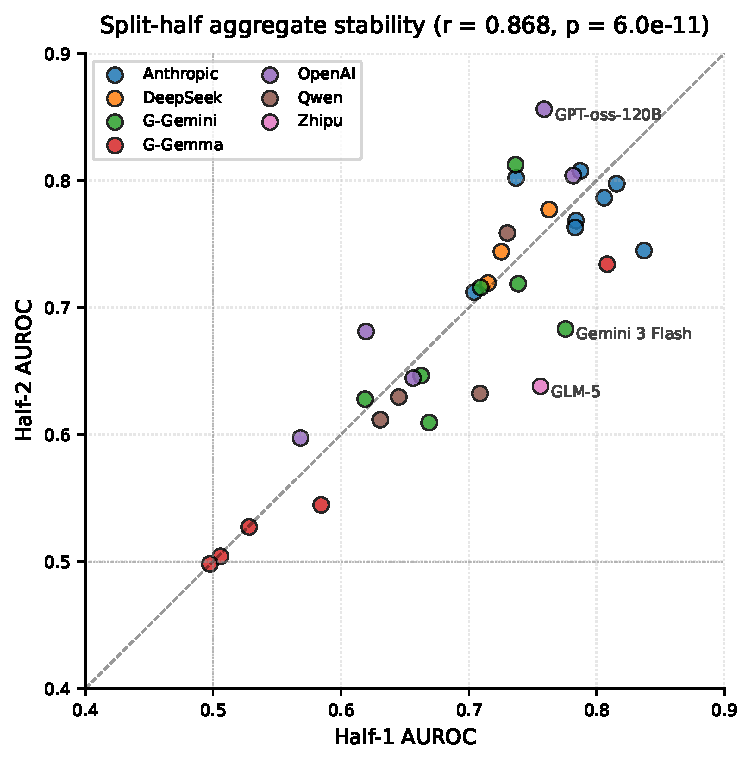
\includegraphics[width=0.6\textwidth]{fig6_splithalf.pdf}
\caption{Split-half stability of aggregate Type-2 AUROC across 33 models. Each point is one model; axes are AUROC on two random halves of its items. Cross-model $r = .868$.}
\label{fig:splithalf}
\end{figure}

\section{Families and generations}
\label{app:families}

\begin{figure}[!htbp]
\centering
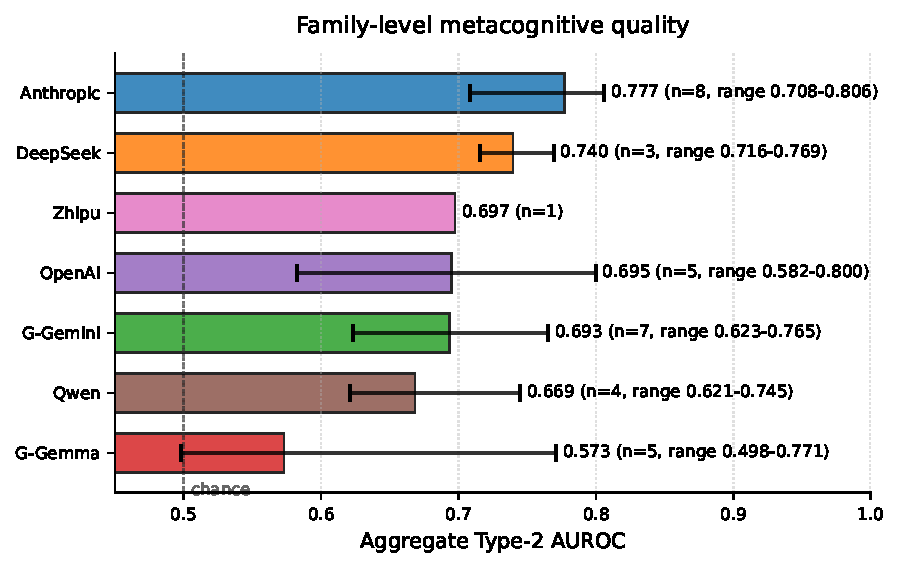
\includegraphics[width=0.7\textwidth]{fig4_family_means.pdf}
\caption{Family mean domain profiles (Type-2 AUROC). Exploratory; see \S\ref{sec:hierarchy} on profile reliability.}
\label{fig:families}
\end{figure}

\textbf{Item-level transitions.} Table~\ref{tab:transitions} cross-classifies shared items by correctness under the earlier and later model in three generational pairs. Per-item confidence correlates more weakly across the Gemma step (Spearman $\rho = .36$) than across Anthropic steps (.75--.85) or DeepSeek steps (.66--.68).

\begin{table}[!htbp]
\centering
\caption{Correctness transitions on shared items (W = wrong, C = correct; earlier $\to$ later). The last column is the later model's mean confidence on items it newly gets wrong.}
\label{tab:transitions}
\small
\begin{tabular}{lrrrrr}
\toprule
\textbf{Pair} & \textbf{W$\to$W} & \textbf{W$\to$C} & \textbf{C$\to$W} & \textbf{C$\to$C} & \textbf{Conf.\ on C$\to$W} \\
\midrule
Gemma 3 27B $\to$ Gemma 4 31B & 57 & 265 & 32 & 1{,}144 & 90.8 \\
Opus 4.1 $\to$ Opus 4.7 & 49 & 37 & 31 & 1{,}382 & 71.5 \\
DeepSeek V3.2 $\to$ R1 & 71 & 64 & 48 & 1{,}188 & 84.6 \\
\bottomrule
\end{tabular}
\end{table}

\section{GLM-5 retest}
\label{app:glm5}

GLM-5's original run stopped after 598 items. It was rerun on the full item set three months later under the same prompt and settings. Table~\ref{tab:glm5} compares the two runs on the 598 shared items. The six domain values correlate $\rho = .77$ ($p = .072$) and $r = .75$. Correctness agrees on 98.5\% of items, and item-level confidence correlates $r = .71$. In both runs Humanities exceeds Applied. With 2 to 14 errors per domain, neither run's domain estimates are precise.

\begin{table}[!htbp]
\centering
\caption{GLM-5 on the same 598 items in two runs three months apart: errors and Type-2 AUROC per domain.}
\label{tab:glm5}
\small
\begin{tabular}{lrrrrr}
\toprule
& & \multicolumn{2}{c}{\textbf{Original run}} & \multicolumn{2}{c}{\textbf{Rerun}} \\
\cmidrule(lr){3-4}\cmidrule(lr){5-6}
\textbf{Domain} & \textbf{$n$} & \textbf{Errors} & \textbf{AUROC} & \textbf{Errors} & \textbf{AUROC} \\
\midrule
Applied & 84 & 4 & .602 & 5 & .639 \\
Factual & 111 & 8 & .576 & 10 & .702 \\
Formal & 102 & 3 & .609 & 5 & .757 \\
Humanities & 91 & 3 & .818 & 2 & .792 \\
Science & 110 & 3 & .555 & 4 & .709 \\
Social & 100 & 14 & .790 & 12 & .777 \\
\midrule
Aggregate & 598 & 35 & .697 & 38 & .759 \\
\bottomrule
\end{tabular}
\end{table}

\section{Partial runs}
\label{app:partial}

Twelve runs are incomplete because of platform timeouts; the smallest are GLM-5 (598 items) and Gemini 2.5 Pro (981). Four further models fall below 1{,}500 only because of the exclusions in Appendix~\ref{app:parsing}. Whether an item is present was tested against its domain for each incomplete model ($\chi^2$, 5 df). Presence is unrelated to domain ($p > .07$) for every model except Gemma 3 12B ($p = .010$; 54 items missing) and GPT-oss-120B ($p = .003$; Appendix~\ref{app:gptoss}).

\section{Future directions}

\textbf{Transport.} Whether the population-level ordering holds on a benchmark with non-overlapping items (for example GPQA) and under other elicitation formats is the main open question.

\textbf{Mechanism.} Hidden-state analyses of open-weight models (Gemma 4 31B, GPT-oss-20B, Qwen Think) could test whether Applied items produce more separable internal states than Formal items.

\textbf{Precision.} Per-model profiles would need many more errors per cell to be interpretable. For high-accuracy models that means many more items per domain, or harder items.

\textbf{Repair.} Whether targeted fine-tuning with confidence in the training signal can raise discrimination in a model's weakest domain is untested. The Gemma step shows that a large aggregate gain can come from error removal alone (Table~\ref{tab:generational}), so any such test should decompose its effect the same way.

\section{Procedural analogy to clinical assessment}
\label{app:neuropsych}

Clinical neuropsychological assessment follows a fixed interpretive sequence. Validity indicators are checked first \citep{larrabee2012}. If the protocol is valid, aggregate scores give an overall level, and the profile of index scores is then examined for relative strengths and weaknesses. The atlas follows the same order: screen the confidence signal \citep{cacioli2026e}, compute the aggregate, then examine the domain profile. The analogy is procedural only. Human cognitive domains rest on extensive factor-analytic validation; the MMLU bins used here do not, and \S\ref{sec:hierarchy} shows they are not cohesive. The analogy also marks a limit: in clinical practice an index score is interpreted only when its reliability supports it, and at current item counts most per-model domain profiles here do not meet that standard.

\section{Bootstrap intervals and error counts}
\label{app:ci}

Table~\ref{tab:s1} gives bootstrap 95\% intervals and error counts for all 198 model-domain cells. Median interval width is .202.

\begin{longtable}{llrrrrr}
\caption{Bootstrap 95\% confidence intervals and error counts for all 198 model-domain AUROC cells (1{,}000 resamples per cell, seeded per cell). Median CI width = .202. Archived as \texttt{data/atlas\_bootstrap\_cis.csv} and \texttt{data/atlas\_cell\_error\_counts.csv}.} \label{tab:s1} \\
\toprule
\textbf{Model} & \textbf{Domain} & \textbf{n} & \textbf{Errors} & \textbf{AUROC} & \textbf{CI lo} & \textbf{CI hi} \\
\midrule
\endfirsthead
\multicolumn{7}{c}{\tablename\ \thetable\ -- continued} \\
\toprule
\textbf{Model} & \textbf{Domain} & \textbf{n} & \textbf{Errors} & \textbf{AUROC} & \textbf{CI lo} & \textbf{CI hi} \\
\midrule
\endhead
\midrule
\multicolumn{7}{r}{{Continued on next page}} \\
\endfoot
\bottomrule
\endlastfoot
Opus 4.6 & Applied & 250 & 18 & 0.847 & 0.765 & 0.923 \\
Opus 4.6 & Factual & 250 & 15 & 0.818 & 0.694 & 0.927 \\
Opus 4.6 & Human. & 250 & 8 & 0.704 & 0.421 & 0.940 \\
Opus 4.6 & Social & 250 & 12 & 0.873 & 0.800 & 0.938 \\
Opus 4.6 & Formal & 250 & 8 & 0.743 & 0.446 & 0.977 \\
Opus 4.6 & Science & 250 & 13 & 0.758 & 0.623 & 0.886 \\
Opus 4.5 & Applied & 250 & 18 & 0.821 & 0.736 & 0.893 \\
Opus 4.5 & Factual & 250 & 16 & 0.795 & 0.657 & 0.907 \\
Opus 4.5 & Human. & 250 & 8 & 0.678 & 0.409 & 0.919 \\
Opus 4.5 & Social & 250 & 14 & 0.867 & 0.759 & 0.946 \\
Opus 4.5 & Formal & 250 & 10 & 0.787 & 0.565 & 0.950 \\
Opus 4.5 & Science & 250 & 13 & 0.764 & 0.629 & 0.884 \\
Sonnet 4.5 & Applied & 250 & 26 & 0.849 & 0.781 & 0.910 \\
Sonnet 4.5 & Factual & 250 & 13 & 0.709 & 0.528 & 0.857 \\
Sonnet 4.5 & Human. & 250 & 7 & 0.715 & 0.464 & 0.915 \\
Sonnet 4.5 & Social & 250 & 16 & 0.801 & 0.708 & 0.889 \\
Sonnet 4.5 & Formal & 250 & 7 & 0.752 & 0.507 & 0.989 \\
Sonnet 4.5 & Science & 250 & 12 & 0.758 & 0.593 & 0.925 \\
Opus 4.7 & Applied & 250 & 19 & 0.853 & 0.764 & 0.917 \\
Opus 4.7 & Factual & 249 & 14 & 0.726 & 0.581 & 0.868 \\
Opus 4.7 & Human. & 250 & 7 & 0.692 & 0.389 & 0.970 \\
Opus 4.7 & Social & 250 & 17 & 0.825 & 0.735 & 0.895 \\
Opus 4.7 & Formal & 250 & 12 & 0.780 & 0.592 & 0.943 \\
Opus 4.7 & Science & 250 & 11 & 0.817 & 0.677 & 0.934 \\
Sonnet 4.6 & Applied & 250 & 20 & 0.887 & 0.822 & 0.940 \\
Sonnet 4.6 & Factual & 250 & 17 & 0.780 & 0.646 & 0.903 \\
Sonnet 4.6 & Human. & 250 & 13 & 0.760 & 0.578 & 0.916 \\
Sonnet 4.6 & Social & 250 & 27 & 0.694 & 0.598 & 0.784 \\
Sonnet 4.6 & Formal & 250 & 8 & 0.788 & 0.540 & 0.976 \\
Sonnet 4.6 & Science & 250 & 12 & 0.782 & 0.629 & 0.906 \\
Sonnet 4 & Applied & 250 & 21 & 0.828 & 0.766 & 0.888 \\
Sonnet 4 & Factual & 250 & 16 & 0.683 & 0.543 & 0.815 \\
Sonnet 4 & Human. & 250 & 13 & 0.756 & 0.616 & 0.873 \\
Sonnet 4 & Social & 250 & 21 & 0.794 & 0.698 & 0.866 \\
Sonnet 4 & Formal & 250 & 9 & 0.735 & 0.558 & 0.915 \\
Sonnet 4 & Science & 250 & 16 & 0.786 & 0.665 & 0.893 \\
Haiku 4.5 & Applied & 248 & 28 & 0.829 & 0.743 & 0.907 \\
Haiku 4.5 & Factual & 250 & 26 & 0.720 & 0.610 & 0.819 \\
Haiku 4.5 & Human. & 250 & 11 & 0.793 & 0.645 & 0.915 \\
Haiku 4.5 & Social & 250 & 28 & 0.728 & 0.638 & 0.810 \\
Haiku 4.5 & Formal & 250 & 17 & 0.805 & 0.663 & 0.923 \\
Haiku 4.5 & Science & 250 & 16 & 0.706 & 0.567 & 0.838 \\
Opus 4.1 & Applied & 250 & 18 & 0.838 & 0.781 & 0.889 \\
Opus 4.1 & Factual & 250 & 11 & 0.615 & 0.444 & 0.775 \\
Opus 4.1 & Human. & 250 & 7 & 0.711 & 0.479 & 0.924 \\
Opus 4.1 & Social & 250 & 20 & 0.781 & 0.682 & 0.867 \\
Opus 4.1 & Formal & 250 & 12 & 0.691 & 0.521 & 0.840 \\
Opus 4.1 & Science & 250 & 18 & 0.636 & 0.526 & 0.761 \\
DeepSeek-R1 & Applied & 250 & 27 & 0.843 & 0.775 & 0.907 \\
DeepSeek-R1 & Factual & 250 & 20 & 0.682 & 0.539 & 0.815 \\
DeepSeek-R1 & Human. & 250 & 14 & 0.785 & 0.635 & 0.922 \\
DeepSeek-R1 & Social & 250 & 33 & 0.814 & 0.725 & 0.889 \\
DeepSeek-R1 & Formal & 250 & 13 & 0.745 & 0.596 & 0.875 \\
DeepSeek-R1 & Science & 250 & 20 & 0.694 & 0.540 & 0.830 \\
DeepSeek V3.2 & Applied & 228 & 31 & 0.713 & 0.612 & 0.803 \\
DeepSeek V3.2 & Factual & 221 & 23 & 0.769 & 0.683 & 0.849 \\
DeepSeek V3.2 & Human. & 229 & 13 & 0.698 & 0.562 & 0.817 \\
DeepSeek V3.2 & Social & 231 & 36 & 0.669 & 0.576 & 0.751 \\
DeepSeek V3.2 & Formal & 231 & 13 & 0.769 & 0.607 & 0.901 \\
DeepSeek V3.2 & Science & 231 & 19 & 0.697 & 0.557 & 0.811 \\
DeepSeek V3.1 & Applied & 234 & 44 & 0.756 & 0.681 & 0.820 \\
DeepSeek V3.1 & Factual & 229 & 22 & 0.690 & 0.578 & 0.799 \\
DeepSeek V3.1 & Human. & 230 & 20 & 0.717 & 0.591 & 0.825 \\
DeepSeek V3.1 & Social & 225 & 38 & 0.636 & 0.531 & 0.728 \\
DeepSeek V3.1 & Formal & 228 & 24 & 0.797 & 0.691 & 0.888 \\
DeepSeek V3.1 & Science & 234 & 29 & 0.626 & 0.514 & 0.733 \\
Gemini 3.1 Pro & Applied & 227 & 13 & 0.841 & 0.715 & 0.949 \\
Gemini 3.1 Pro & Factual & 215 & 14 & 0.773 & 0.629 & 0.899 \\
Gemini 3.1 Pro & Human. & 228 & 8 & 0.764 & 0.533 & 0.972 \\
Gemini 3.1 Pro & Social & 225 & 19 & 0.776 & 0.663 & 0.883 \\
Gemini 3.1 Pro & Formal & 230 & 6 & 0.645 & 0.469 & 0.891 \\
Gemini 3.1 Pro & Science & 221 & 9 & 0.640 & 0.467 & 0.826 \\
Gemini 3 Flash & Applied & 250 & 13 & 0.800 & 0.718 & 0.881 \\
Gemini 3 Flash & Factual & 250 & 13 & 0.673 & 0.516 & 0.825 \\
Gemini 3 Flash & Human. & 250 & 9 & 0.662 & 0.496 & 0.829 \\
Gemini 3 Flash & Social & 250 & 17 & 0.794 & 0.693 & 0.879 \\
Gemini 3 Flash & Formal & 250 & 9 & 0.681 & 0.504 & 0.862 \\
Gemini 3 Flash & Science & 250 & 12 & 0.690 & 0.530 & 0.845 \\
Gemini 2.5 Flash & Applied & 227 & 28 & 0.801 & 0.709 & 0.880 \\
Gemini 2.5 Flash & Factual & 219 & 20 & 0.765 & 0.638 & 0.883 \\
Gemini 2.5 Flash & Human. & 231 & 12 & 0.644 & 0.485 & 0.807 \\
Gemini 2.5 Flash & Social & 228 & 32 & 0.748 & 0.661 & 0.835 \\
Gemini 2.5 Flash & Formal & 230 & 19 & 0.637 & 0.534 & 0.745 \\
Gemini 2.5 Flash & Science & 225 & 16 & 0.664 & 0.546 & 0.800 \\
Gemini 2.5 Pro & Applied & 165 & 17 & 0.889 & 0.794 & 0.960 \\
Gemini 2.5 Pro & Factual & 172 & 11 & 0.619 & 0.484 & 0.788 \\
Gemini 2.5 Pro & Human. & 160 & 6 & 0.623 & 0.449 & 0.844 \\
Gemini 2.5 Pro & Social & 150 & 15 & 0.754 & 0.623 & 0.893 \\
Gemini 2.5 Pro & Formal & 163 & 6 & 0.573 & 0.478 & 0.777 \\
Gemini 2.5 Pro & Science & 171 & 7 & 0.485 & 0.469 & 0.497 \\
Gemini 3.1 FLite & Applied & 231 & 28 & 0.823 & 0.737 & 0.898 \\
Gemini 3.1 FLite & Factual & 233 & 18 & 0.752 & 0.636 & 0.858 \\
Gemini 3.1 FLite & Human. & 222 & 9 & 0.651 & 0.471 & 0.841 \\
Gemini 3.1 FLite & Social & 229 & 29 & 0.624 & 0.531 & 0.714 \\
Gemini 3.1 FLite & Formal & 227 & 31 & 0.566 & 0.506 & 0.641 \\
Gemini 3.1 FLite & Science & 223 & 19 & 0.549 & 0.474 & 0.646 \\
Gemini 2.0 FLite & Applied & 250 & 56 & 0.688 & 0.623 & 0.749 \\
Gemini 2.0 FLite & Factual & 250 & 35 & 0.692 & 0.585 & 0.777 \\
Gemini 2.0 FLite & Human. & 250 & 25 & 0.662 & 0.547 & 0.769 \\
Gemini 2.0 FLite & Social & 250 & 48 & 0.555 & 0.468 & 0.646 \\
Gemini 2.0 FLite & Formal & 250 & 61 & 0.667 & 0.597 & 0.740 \\
Gemini 2.0 FLite & Science & 250 & 45 & 0.621 & 0.533 & 0.711 \\
Gemini 2.0 Flash & Applied & 250 & 45 & 0.758 & 0.691 & 0.822 \\
Gemini 2.0 Flash & Factual & 250 & 29 & 0.732 & 0.629 & 0.822 \\
Gemini 2.0 Flash & Human. & 250 & 13 & 0.663 & 0.512 & 0.808 \\
Gemini 2.0 Flash & Social & 250 & 41 & 0.503 & 0.420 & 0.583 \\
Gemini 2.0 Flash & Formal & 250 & 43 & 0.572 & 0.498 & 0.648 \\
Gemini 2.0 Flash & Science & 250 & 30 & 0.606 & 0.505 & 0.696 \\
Gemma 4 31B & Applied & 250 & 17 & 0.869 & 0.773 & 0.942 \\
Gemma 4 31B & Factual & 250 & 19 & 0.663 & 0.535 & 0.792 \\
Gemma 4 31B & Human. & 250 & 11 & 0.737 & 0.564 & 0.889 \\
Gemma 4 31B & Social & 250 & 23 & 0.806 & 0.703 & 0.904 \\
Gemma 4 31B & Formal & 250 & 9 & 0.812 & 0.638 & 0.981 \\
Gemma 4 31B & Science & 250 & 12 & 0.710 & 0.558 & 0.856 \\
Gemma 3 27B & Applied & 248 & 67 & 0.585 & 0.526 & 0.646 \\
Gemma 3 27B & Factual & 250 & 37 & 0.674 & 0.599 & 0.748 \\
Gemma 3 27B & Human. & 249 & 24 & 0.573 & 0.488 & 0.665 \\
Gemma 3 27B & Social & 250 & 54 & 0.528 & 0.468 & 0.583 \\
Gemma 3 27B & Formal & 250 & 76 & 0.569 & 0.500 & 0.634 \\
Gemma 3 27B & Science & 250 & 63 & 0.598 & 0.543 & 0.645 \\
Gemma 3 4B & Applied & 244 & 118 & 0.536 & 0.485 & 0.585 \\
Gemma 3 4B & Factual & 241 & 65 & 0.564 & 0.494 & 0.637 \\
Gemma 3 4B & Human. & 240 & 55 & 0.506 & 0.441 & 0.562 \\
Gemma 3 4B & Social & 240 & 113 & 0.488 & 0.430 & 0.543 \\
Gemma 3 4B & Formal & 239 & 131 & 0.541 & 0.483 & 0.609 \\
Gemma 3 4B & Science & 241 & 112 & 0.566 & 0.507 & 0.621 \\
Gemma 3 12B & Applied & 242 & 77 & 0.533 & 0.463 & 0.601 \\
Gemma 3 12B & Factual & 237 & 47 & 0.614 & 0.522 & 0.696 \\
Gemma 3 12B & Human. & 243 & 29 & 0.522 & 0.420 & 0.625 \\
Gemma 3 12B & Social & 247 & 71 & 0.464 & 0.392 & 0.537 \\
Gemma 3 12B & Formal & 233 & 99 & 0.554 & 0.502 & 0.605 \\
Gemma 3 12B & Science & 244 & 66 & 0.500 & 0.430 & 0.575 \\
Gemma 3 1B & Applied & 249 & 163 & 0.495 & 0.465 & 0.524 \\
Gemma 3 1B & Factual & 250 & 124 & 0.501 & 0.472 & 0.531 \\
Gemma 3 1B & Human. & 250 & 112 & 0.500 & 0.476 & 0.523 \\
Gemma 3 1B & Social & 250 & 161 & 0.490 & 0.463 & 0.514 \\
Gemma 3 1B & Formal & 250 & 185 & 0.503 & 0.477 & 0.527 \\
Gemma 3 1B & Science & 250 & 172 & 0.502 & 0.479 & 0.520 \\
GPT-oss-120B & Applied & 93 & 18 & 0.829 & 0.742 & 0.902 \\
GPT-oss-120B & Factual & 65 & 7 & 0.855 & 0.625 & 0.989 \\
GPT-oss-120B & Human. & 81 & 5 & 0.611 & 0.244 & 0.925 \\
GPT-oss-120B & Social & 78 & 11 & 0.801 & 0.659 & 0.923 \\
GPT-oss-120B & Formal & 99 & 2 & 0.515 & 0.128 & 0.918 \\
GPT-oss-120B & Science & 102 & 11 & 0.760 & 0.582 & 0.900 \\
GPT-oss-20B & Applied & 250 & 57 & 0.769 & 0.697 & 0.827 \\
GPT-oss-20B & Factual & 250 & 34 & 0.766 & 0.675 & 0.847 \\
GPT-oss-20B & Human. & 250 & 25 & 0.803 & 0.688 & 0.904 \\
GPT-oss-20B & Social & 250 & 27 & 0.827 & 0.745 & 0.901 \\
GPT-oss-20B & Formal & 250 & 16 & 0.758 & 0.588 & 0.896 \\
GPT-oss-20B & Science & 250 & 20 & 0.709 & 0.592 & 0.810 \\
GPT-5.4 mini & Applied & 227 & 45 & 0.743 & 0.649 & 0.821 \\
GPT-5.4 mini & Factual & 216 & 26 & 0.797 & 0.712 & 0.870 \\
GPT-5.4 mini & Human. & 230 & 14 & 0.723 & 0.598 & 0.834 \\
GPT-5.4 mini & Social & 228 & 55 & 0.604 & 0.508 & 0.693 \\
GPT-5.4 mini & Formal & 232 & 64 & 0.572 & 0.492 & 0.649 \\
GPT-5.4 mini & Science & 223 & 41 & 0.725 & 0.631 & 0.815 \\
GPT-5.4 & Applied & 250 & 29 & 0.818 & 0.735 & 0.887 \\
GPT-5.4 & Factual & 250 & 21 & 0.777 & 0.652 & 0.880 \\
GPT-5.4 & Human. & 250 & 11 & 0.640 & 0.397 & 0.876 \\
GPT-5.4 & Social & 250 & 27 & 0.747 & 0.638 & 0.849 \\
GPT-5.4 & Formal & 250 & 41 & 0.539 & 0.452 & 0.631 \\
GPT-5.4 & Science & 250 & 28 & 0.649 & 0.533 & 0.754 \\
GPT-5.4 nano & Applied & 250 & 85 & 0.633 & 0.565 & 0.700 \\
GPT-5.4 nano & Factual & 250 & 58 & 0.749 & 0.674 & 0.813 \\
GPT-5.4 nano & Human. & 250 & 50 & 0.726 & 0.652 & 0.798 \\
GPT-5.4 nano & Social & 250 & 100 & 0.486 & 0.410 & 0.564 \\
GPT-5.4 nano & Formal & 250 & 132 & 0.548 & 0.477 & 0.620 \\
GPT-5.4 nano & Science & 250 & 95 & 0.615 & 0.538 & 0.691 \\
Qwen Think & Applied & 250 & 22 & 0.726 & 0.611 & 0.838 \\
Qwen Think & Factual & 250 & 18 & 0.680 & 0.528 & 0.811 \\
Qwen Think & Human. & 250 & 10 & 0.714 & 0.529 & 0.875 \\
Qwen Think & Social & 250 & 32 & 0.768 & 0.695 & 0.836 \\
Qwen Think & Formal & 250 & 8 & 0.644 & 0.443 & 0.838 \\
Qwen Think & Science & 250 & 14 & 0.757 & 0.630 & 0.877 \\
Qwen Coder & Applied & 250 & 49 & 0.650 & 0.585 & 0.716 \\
Qwen Coder & Factual & 250 & 29 & 0.716 & 0.637 & 0.791 \\
Qwen Coder & Human. & 250 & 16 & 0.723 & 0.597 & 0.827 \\
Qwen Coder & Social & 250 & 51 & 0.616 & 0.540 & 0.688 \\
Qwen Coder & Formal & 250 & 23 & 0.576 & 0.459 & 0.690 \\
Qwen Coder & Science & 250 & 28 & 0.696 & 0.603 & 0.794 \\
Qwen 80B Inst & Applied & 250 & 45 & 0.647 & 0.571 & 0.723 \\
Qwen 80B Inst & Factual & 249 & 28 & 0.667 & 0.571 & 0.770 \\
Qwen 80B Inst & Human. & 250 & 12 & 0.716 & 0.564 & 0.854 \\
Qwen 80B Inst & Social & 250 & 49 & 0.691 & 0.621 & 0.759 \\
Qwen 80B Inst & Formal & 250 & 46 & 0.585 & 0.516 & 0.671 \\
Qwen 80B Inst & Science & 249 & 35 & 0.584 & 0.483 & 0.680 \\
Qwen 235B & Applied & 250 & 55 & 0.644 & 0.581 & 0.711 \\
Qwen 235B & Factual & 250 & 23 & 0.622 & 0.522 & 0.728 \\
Qwen 235B & Human. & 250 & 16 & 0.711 & 0.601 & 0.827 \\
Qwen 235B & Social & 250 & 33 & 0.650 & 0.538 & 0.740 \\
Qwen 235B & Formal & 250 & 42 & 0.567 & 0.478 & 0.655 \\
Qwen 235B & Science & 250 & 32 & 0.637 & 0.573 & 0.695 \\
GLM-5 & Applied & 84 & 4 & 0.602 & 0.221 & 0.916 \\
GLM-5 & Factual & 111 & 8 & 0.576 & 0.399 & 0.775 \\
GLM-5 & Human. & 91 & 3 & 0.818 & 0.706 & 0.972 \\
GLM-5 & Social & 100 & 14 & 0.790 & 0.648 & 0.908 \\
GLM-5 & Formal & 102 & 3 & 0.609 & 0.388 & 1.000 \\
GLM-5 & Science & 110 & 3 & 0.554 & 0.387 & 0.853 \\
\end{longtable}

